\begin{center}
    \Huge{\textbf{\underline{I.Exercise 1}}}
\end{center}

\vspace{0.45cm}

\begin{center}
    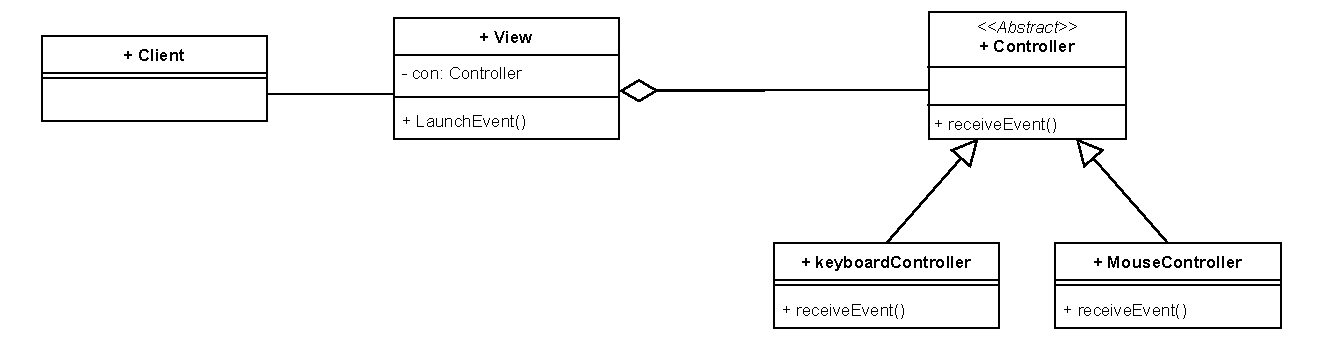
\includegraphics[height=0.16\textheight]{Exercices/1.EX1/ex1.drawio.pdf}
\end{center}

\vspace{0.25cm}

\begin{prettyBox}{Explication}{myblue}
The context here is the \texttt{View} class, since that's what the user interacts with. 
From there, the user can trigger different interchangeable events that will be 
handled accordingly by the controller. Therefore, the controller is the \texttt{Strategy} class, 
and in general we can have an event trigged from the mouse or from the keyboard
\end{prettyBox}

